\section{Resultados} \label{results}

% deve
% • apresentar uma descrição detalhada dos dados coletados de modo que aqueles que estiverem lendo o trabalho possam ter a exata dimensão do que foi apreendido na pesquisa.
% • os dados podem ser apresentados em forma de tabelas, quadros, gráficos e outras figuras ilustrativas como fluxos, esquemas, etc., que devem ser inseridos o mais próximo possível do trecho do texto no qual se inicia a descrição dos principais resultados apresentados na figura.

Com a alteração do fluxo de trabalho para ser iniciado em uma atividade escolhida pelo usuários, podemos visualizar na figura \ref{fig:changedWorkflow} o novo fluxo de trabalho, indicando o corte do workflow na atividade selecionada, transformando a atividade selecionada em um novo ponto de inicio e adicionando uma nova atividade inicial no fluxo de trabalho. Assim, caso o usuário queira acesso à atividades anteriores para obter informações que podem ser necessárias para a nova atividade inicial ou para futuras atividades, ele pode visualizar estas informações acessando o flux dividido, enquanto que para acessar próximas atividades e poder criar novas atividades, o usuário pode seguir no novo fluxo principal.

No caso do workflow CENTRARE, podemos ver pela figura \ref{fig:changedInstance} que, ao selecionarmos uma nova atividade inicial, temos mais funcionalidades na hora de selecionar qual atividade realmente queremos acessar (com a disponibilização de busca de atributos da atividade, busca por nome da atividade ou data de criação), além de diminuir consideravelmente o número de cliques que o usuário deve fazer para acessar a atividade (figura \ref{fig:changedWorkflow}).

\begin{figure}
    \centering
    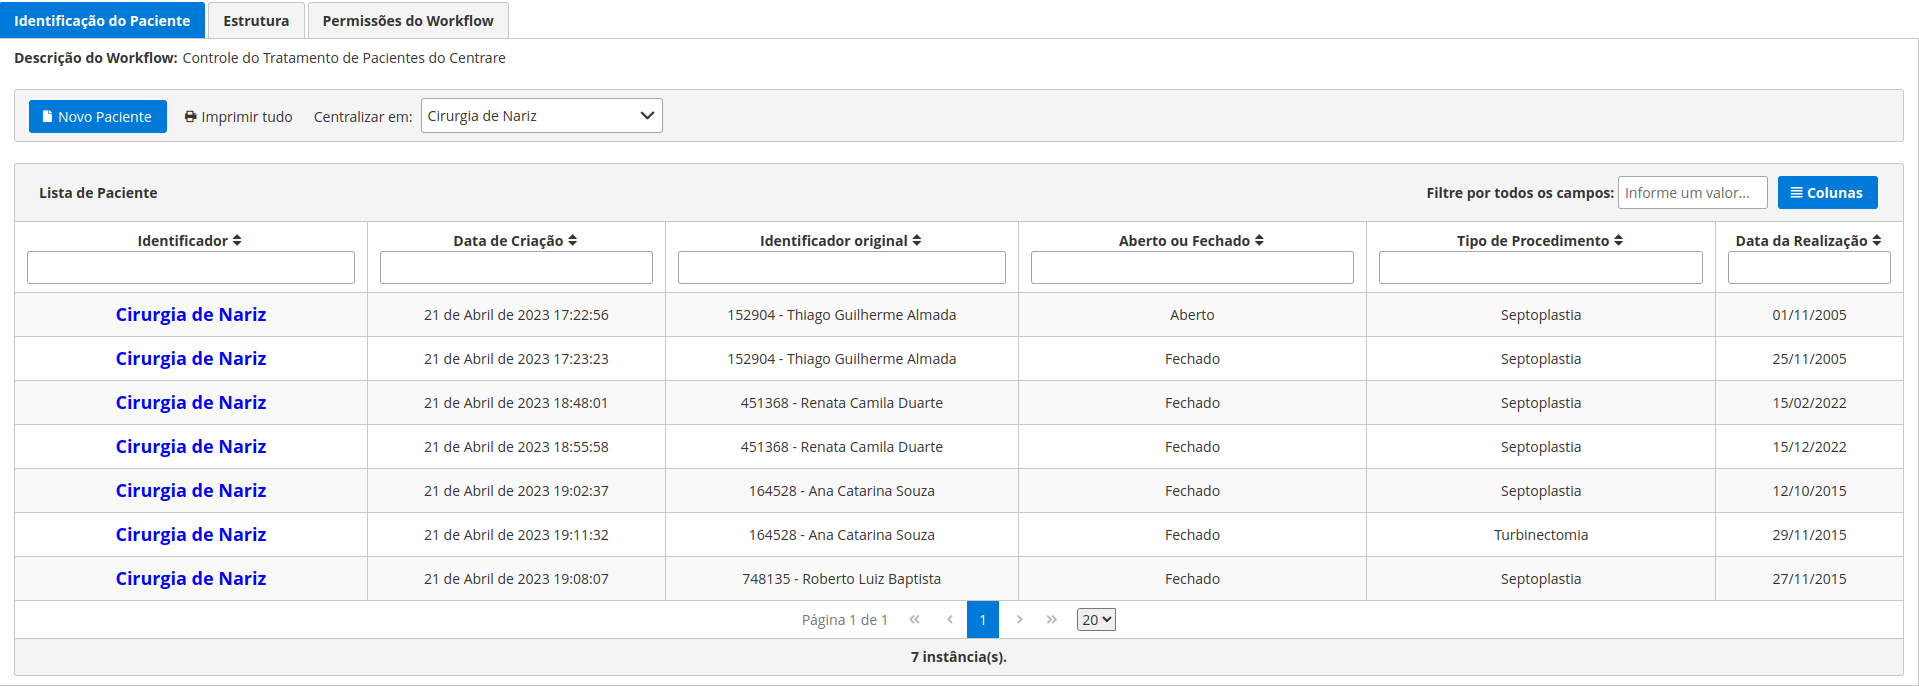
\includegraphics[width=1\textwidth]{imgs/CENTRARE/instanciaAlterada.png}
    \caption{Lista de instâncias do workflow CENTRARE, centralizado na atividade "Cirurgia de nariz"}
    \label{fig:changedInstance}
\end{figure}

Com a modificação da árvore de atividades, temos também a divisão de informações que limpa a tela para o usuário, retirando parte das informações parcialmente desnecessárias que o usuário teria que navegar para chegar na atividade que será preenchida no momento.

Como uma das maiores reclamações em softwares de teleatendimento e de softwares de manejamento de laboratórios é uma experiência de usuário confusa, sem levar em conta o contexto do usuário na ferramenta nem do que o usuário necessita dentro da ferramenta para obter um resultado em suas atividades, o remanejo de atividades em um BPM facilita a utilização da ferramenta e, com isso, aumenta a eficiência da utilização do software.

No caso do workflow BPL, temos que os benefícios não são muito aparentes pelo tamanho do workflow e também pelo número de instâncias que são criadas (disponibilizando informações para preenchimento com sua atividade inicial original). Isso faz com que a consulta de atividades se torne mais fácil e não existem muitas informações que podem ficar omitidas atrás de muitas atividades.

No caso do workflow CENTRARE, a centralização de atividades foi muito benéfica, já que o workflow tem uma profundidade considerável e o número de pessoas que trabalham nesse workflow também é grande. Com a centralização, encontrar atividades que são interessantes para o usuário em determinado momento é uma questão de selecionar a atividade a ser selecionada e fazer a busca dos dados pelos atributos da atividade escolhida.

Como a identificação original do workflow é pelo paciente, que pode ter uma ou mais cirurgias, para que o médico encontre uma cirurgia específica, ele apenas centraliza o workflow na atividade da cirurgia desejada e procura pelos atributos desejados, sem que precise lembrar de qual paciente foi a cirurgia.

Para o compartilhamento de informações, o CENTRARE poderia ser dividido em vários workflows separados para cada tipo de funcionário (nutricionista, psicologo, fonoaudiologo) e, com o compartilhamento de informações entre workflows, um novo workflow poderia ser montado com esta divisão em mente e haver uma maior separação de informações entre os profissionais, mantendo apenas informações importantes disponíveis para cada um.

No BPL, como já dito, temos o compartilhamento de mensagens entre técnicos e cientistas para obter informações de equipamentos e experimentos realizados, além dos gerentes de laboratório tendo as duas informações condensadas em um só lugar.

Há também, para futuros BPMs implementados, o controle de estoque facilitado com troca de informações (como um laboratório que compartilha racks com outro laboratório e necessita da informação de disponibilidade, mantendo sempre essa informação atualizada entre laboratórios)